
\documentclass[11pt,a4paper]{article}
\usepackage[T1]{fontenc}
\usepackage{lmodern}
\usepackage{amsmath,amssymb,amsfonts,mathtools}
\usepackage{graphicx,booktabs,longtable,array,tabularx,adjustbox}
\usepackage{geometry,microtype,fancyhdr,lastpage,etoolbox,enumitem}
\usepackage{newunicodechar,textcomp}
\usepackage{hyperref}
\hypersetup{hidelinks,pdfcreator={XeLaTeX / QM1 academic edition}}
\geometry{left=20mm,right=20mm,top=22mm,bottom=23mm}
\setcounter{secnumdepth}{2}
\setlength{\parindent}{0pt}
\setlength{\parskip}{4pt plus 1pt}
\setlength{\emergencystretch}{2em}
\setlength{\tabcolsep}{3pt}
\renewcommand{\arraystretch}{1.16}
\setlist{nosep,topsep=3pt,itemsep=2pt,leftmargin=7mm}
\AtBeginEnvironment{longtable}{\footnotesize\setlength{\tabcolsep}{2.2pt}}
\newcommand{\tightlist}{\setlength{\itemsep}{0pt}\setlength{\parskip}{0pt}}
\providecommand{\Cov}{\operatorname{Cov}}
\providecommand{\Var}{\operatorname{Var}}
\providecommand{\Corr}{\operatorname{Corr}}
\providecommand{\MAD}{\operatorname{MAD}}
\providecommand{\E}{\mathbb{E}}
\providecommand{\R}{\mathbb{R}}
\newunicodechar{—}{\textemdash}
\newunicodechar{–}{\textendash}
\newunicodechar{€}{\texteuro}
\newunicodechar{≤}{\ensuremath{\leq}}
\newunicodechar{≥}{\ensuremath{\geq}}
\newunicodechar{×}{\ensuremath{\times}}
\newunicodechar{÷}{\ensuremath{\div}}
\newunicodechar{Σ}{\ensuremath{\Sigma}}
\newunicodechar{σ}{\ensuremath{\sigma}}
\newunicodechar{μ}{\ensuremath{\mu}}
\newunicodechar{Δ}{\ensuremath{\Delta}}
\newunicodechar{∑}{\ensuremath{\sum}}
\newunicodechar{≈}{\ensuremath{\approx}}
\newunicodechar{√}{\ensuremath{\surd}}
\newunicodechar{≠}{\ensuremath{\ne}}
\newunicodechar{→}{\ensuremath{\to}}
\newunicodechar{∞}{\ensuremath{\infty}}
\newunicodechar{∈}{\ensuremath{\in}}
\newunicodechar{−}{\ensuremath{-}}
\newunicodechar{²}{\ensuremath{^{2}}}
\newunicodechar{³}{\ensuremath{^{3}}}
\newunicodechar{₀}{\ensuremath{_{0}}}
\newunicodechar{₁}{\ensuremath{_{1}}}
\newunicodechar{₂}{\ensuremath{_{2}}}
\newunicodechar{₃}{\ensuremath{_{3}}}
\newunicodechar{₄}{\ensuremath{_{4}}}
\newunicodechar{ₜ}{\ensuremath{_{t}}}
\newunicodechar{ₚ}{\ensuremath{_{p}}}
\newunicodechar{ₙ}{\ensuremath{_{n}}}
\newunicodechar{ₓ}{\ensuremath{_{x}}}
\newunicodechar{ᵢ}{\ensuremath{_{i}}}
\newunicodechar{ŷ}{\ensuremath{\hat y}}
\newunicodechar{Ŷ}{\ensuremath{\widehat Y}}
\newunicodechar{ₘ}{\ensuremath{_{m}}}
\newunicodechar{ₑ}{\ensuremath{_{e}}}
\newunicodechar{ₐ}{\ensuremath{_{a}}}
\newunicodechar{ₖ}{\ensuremath{_{k}}}
\newunicodechar{ₛ}{\ensuremath{_{s}}}
\newunicodechar{ₗ}{\ensuremath{_{l}}}
\newunicodechar{ₕ}{\ensuremath{_{h}}}
\newunicodechar{ₒ}{\ensuremath{_{o}}}
\newunicodechar{₊}{\ensuremath{_{+}}}
\newunicodechar{₋}{\ensuremath{_{-}}}
\newunicodechar{₌}{\ensuremath{_{=}}}
\newunicodechar{₍}{\ensuremath{_{(}}}
\newunicodechar{₎}{\ensuremath{_{)}}}
\newunicodechar{⁻}{\ensuremath{^{-}}}
\newunicodechar{⁺}{\ensuremath{^{+}}}
\newunicodechar{⁰}{\ensuremath{^{0}}}
\newunicodechar{¹}{\ensuremath{^{1}}}
\newunicodechar{⁴}{\ensuremath{^{4}}}
\newunicodechar{⁵}{\ensuremath{^{5}}}
\newunicodechar{⁶}{\ensuremath{^{6}}}
\newunicodechar{⁷}{\ensuremath{^{7}}}
\newunicodechar{⁸}{\ensuremath{^{8}}}
\newunicodechar{⁹}{\ensuremath{^{9}}}
\makeatletter
\renewcommand{\section}{\@startsection{section}{1}{0pt}{2.0ex plus .7ex minus .3ex}{1.0ex}{\large\bfseries}}
\renewcommand{\subsection}{\@startsection{subsection}{2}{0pt}{1.8ex plus .5ex minus .2ex}{.7ex}{\normalsize\bfseries}}
\renewcommand{\subsubsection}{\@startsection{subsubsection}{3}{0pt}{1.3ex plus .4ex minus .2ex}{.5ex}{\normalsize\bfseries}}
\makeatother
\pagestyle{fancy}
\fancyhf{}
\renewcommand{\headrulewidth}{0.35pt}
\renewcommand{\footrulewidth}{0pt}
\fancyhead[L]{\small\textsc{KEDGE Business School --- QM1}}
\fancyhead[R]{\small\textsc{2026--2027}}
\fancyfoot[L]{\small Badr ABOUFARASSE, PhD}
\fancyfoot[R]{\small\thepage\ /\ \pageref{LastPage}}
\setlength{\headheight}{14pt}
\setkeys{Gin}{keepaspectratio}
\begin{document}

\begin{center}
{\small\textsc{KEDGE Business School \quad EBP1 \quad Quantitative Methods 1}}\\[6pt]
{\Large\bfseries Worksheet 5 — Time series}\\[6pt]
{\normalsize\bfseries Fully worked solutions}\\[6pt]
{\small Badr ABOUFARASSE, PhD \quad --- \quad 2026--2027}
\end{center}
\vspace{2mm}\hrule\vspace{6mm}

\hypertarget{core-applications}{%
\section{Core applications}\label{core-applications}}

Master the essential definitions and calculations from the course.

\emph{Core application --- 10 min}

\hypertarget{exercise-1-components-and-models}{%
\subsection{Exercise 1 -- Components and models}\label{exercise-1-components-and-models}}

\begin{enumerate}
\item
  Match long-run trend, recession, recurring Q4 peak and exceptional shock to {\(T_t\)}, {\(C_t\)}, {\(S_t\)} or {\(R_t\)}.
\item
  Write the full additive and multiplicative models.
\item
  Explain when multiplicative seasonality is more plausible than additive seasonality.
\end{enumerate}

\hypertarget{fully-worked-solution}{%
\subsubsection{Fully worked solution}\label{fully-worked-solution}}

{\[Y_t=T_t+C_t+S_t+R_t,\]} {\[Y_t=T_t\times C_t\times S_t\times R_t.\]} Multiplicative seasonality is more plausible when seasonal amplitude grows with the level of the series.

\hypertarget{distinguishing-additive-units-from-multiplicative-factors}{%
\subsubsection{Distinguishing additive units from multiplicative factors}\label{distinguishing-additive-units-from-multiplicative-factors}}

An additive seasonal component is measured in units of Y and has a constant absolute amplitude. A multiplicative seasonal component is a factor (e.g. 1.20 for +20\%), so its absolute effect varies with the trend level. A cycle spans longer fluctuations, whereas an irregular shock is not periodic.

\emph{Core application --- 20 min}

\hypertarget{exercise-2-moving-averages-and-centring}{%
\subsection{Exercise 2 -- Moving averages and centring}\label{exercise-2-moving-averages-and-centring}}

Quarterly demand over two years is {\[80,\
100,\ 120,\ 140,\ 88,\ 110,\ 132,\ 154.\]} Describe the main pattern, calculate the five 4-quarter moving averages, centre them for periods 3 to 6, and explain why an even-order moving average must be centred.

\hypertarget{fully-worked-solution-1}{%
\subsubsection{Fully worked solution}\label{fully-worked-solution-1}}

{\[MA_{2.5}=110,\quad MA_{3.5}=112,\quad
MA_{4.5}=114.5,\quad MA_{5.5}=117.5,\quad MA_{6.5}=121.\]} {\[CMA_3=111,\quad CMA_4=113.25,\quad
CMA_5=116,\quad CMA_6=119.25.\]} An even-order moving average lies between two periods, so averaging adjacent moving averages centres the estimate on an observed period.

\hypertarget{moving-average-alignment-table}{%
\subsubsection{Moving-average alignment table}\label{moving-average-alignment-table}}

\begin{longtable}[]{@{}llll@{}}
\toprule\noalign{}
Window & Sum & MA4 & Midpoint \\
\midrule\noalign{}
\endhead
\bottomrule\noalign{}
\endlastfoot
1--4 & 440 & 110 & 2.5 \\
2--5 & 448 & 112 & 3.5 \\
3--6 & 458 & 114.5 & 4.5 \\
4--7 & 470 & 117.5 & 5.5 \\
5--8 & 484 & 121 & 6.5 \\
\end{longtable}

\begin{longtable}[]{@{}lllll@{}}
\toprule\noalign{}
t & 3 & 4 & 5 & 6 \\
\midrule\noalign{}
\endhead
\bottomrule\noalign{}
\endlastfoot
CMA4 & (110+112)/2=111 & (112+114.5)/2=113.25 & (114.5+117.5)/2=116 & (117.5+121)/2=119.25 \\
\end{longtable}

Because order 4 is even, the first moving average is centred between t=2 and t=3. Centring gives values at integer dates t=3 through 6.

\hypertarget{assessment-and-exam-practice}{%
\section{Assessment and exam practice}\label{assessment-and-exam-practice}}

Practise independently with assessment and final-exam style questions.

\emph{Assessment / exam practice --- 25 min}

\hypertarget{exercise-3-multiplicative-decomposition-and-forecasting}{%
\subsection{Exercise 3 -- Multiplicative decomposition and forecasting}\label{exercise-3-multiplicative-decomposition-and-forecasting}}

\begin{longtable}[]{@{}lllll@{}}
\toprule\noalign{}
Year & Q1 & Q2 & Q3 & Q4 \\
\midrule\noalign{}
\endhead
\bottomrule\noalign{}
\endlastfoot
2005 & 82 & 98 & 120 & 150 \\
2006 & 91 & 111 & 137 & 171 \\
2007 & 104 & 126 & 154 & 194 \\
\end{longtable}

Given {\(\widehat T_t=6.343t+86.939\)} and seasonal coefficients {\(0.789,0.903,1.052,1.255\)}, interpret the trend slope, check normalization, forecast the four quarters of 2008, and explain multiplicative deseasonalization.

\hypertarget{fully-worked-solution-2}{%
\subsubsection{Fully worked solution}\label{fully-worked-solution-2}}

The trend slope 6.343 implies a 6.343-unit increase per quarter. The supplied seasonal factors sum to 3.999, approximately 4 (rounding).

\begin{longtable}[]{@{}lllll@{}}
\toprule\noalign{}
t & Q & Tₜ=6.343t+86.939 & S\textquotesingle{} & Tₜ×S\textquotesingle{} \\
\midrule\noalign{}
\endhead
\bottomrule\noalign{}
\endlastfoot
13 & Q1 & 169.398 & 0.789 & 133.655022 \\
14 & Q2 & 175.741 & 0.903 & 158.694123 \\
15 & Q3 & 182.084 & 1.052 & 191.552368 \\
16 & Q4 & 188.427 & 1.255 & 236.475885 \\
\end{longtable}

\[\widehat Y_{13}=169.398(0.789)=133.655022,\quad\widehat Y_{14}=175.741(0.903)=158.694123.\]

\[\widehat Y_{15}=182.084(1.052)=191.552368,\quad\widehat Y_{16}=188.427(1.255)=236.475885.\]

To deseasonalise an observation, divide Yₜ by the relevant quarterly factor S\textquotesingle. Retain unrounded figures until the final result.

\emph{Assessment / exam practice --- 65 min}

\hypertarget{exercise-5-full-seasonal-decomposition-exam-style}{%
\subsection{Exercise 5 --- Full seasonal decomposition --- exam style}\label{exercise-5-full-seasonal-decomposition-exam-style}}

A firm observes quarterly sales over three years. Use the multiplicative model Yₜ=Tₜ×Sₜ, without explicit cycle or irregular component. Do not round intermediate values.

\begin{longtable}[]{@{}lllll@{}}
\toprule\noalign{}
Année / Year & Q1 & Q2 & Q3 & Q4 \\
\midrule\noalign{}
\endhead
\bottomrule\noalign{}
\endlastfoot
2019 & 40 & 52 & 48 & 68 \\
2020 & 44 & 58 & 53 & 76 \\
2021 & 50 & 65 & 60 & 84 \\
\end{longtable}

\begin{enumerate}
\tightlist
\item
  Plot the series and calculate all nine 4-quarter moving averages.
\item
  Centre the moving averages (t=3 to 10). Build the t, CMA4, t², t×CMA4 table.
\item
  Estimate trend Tₜ=at+b by OLS on the eight centred moving averages.
\item
  Calculate Yₜ/Tₜ for all 12 quarters, the four seasonal means and normalised factors summing to 4.
\item
  Forecast all four quarters of 2022 (t=13 to 16), first deseasonalised, then seasonalised.
\end{enumerate}

\hypertarget{fully-worked-solution-3}{%
\subsubsection{Fully worked solution}\label{fully-worked-solution-3}}

1. Four-quarter moving averages:

\[MA_{2.5}=(40+52+48+68)/4=52,\quad MA_{3.5}=(52+48+68+44)/4=53.\]

\begin{longtable}[]{@{}lllll@{}}
\toprule\noalign{}
Fenêtre / Window & Périodes / Periods & Somme / Sum & MA4 & Centre / Midpoint \\
\midrule\noalign{}
\endhead
\bottomrule\noalign{}
\endlastfoot
1 & 1--4 & 208 & 52 & 2.5 \\
2 & 2--5 & 212 & 53 & 3.5 \\
3 & 3--6 & 218 & 54.5 & 4.5 \\
4 & 4--7 & 223 & 55.75 & 5.5 \\
5 & 5--8 & 231 & 57.75 & 6.5 \\
6 & 6--9 & 237 & 59.25 & 7.5 \\
7 & 7--10 & 244 & 61 & 8.5 \\
8 & 8--11 & 251 & 62.75 & 9.5 \\
9 & 9--12 & 259 & 64.75 & 10.5 \\
\end{longtable}

2. Centring: the nine half-period MA4 values produce eight CMA4 values at integer periods 3 to 10.

\[CMA_3=(52+53)/2=52.5,\quad CMA_4=(53+54.5)/2=53.75.\]

\begin{longtable}[]{@{}llll@{}}
\toprule\noalign{}
t & CMA4 & t² & t×CMA4 \\
\midrule\noalign{}
\endhead
\bottomrule\noalign{}
\endlastfoot
3 & 52.5 & 9 & 157.5 \\
4 & 53.75 & 16 & 215 \\
5 & 55.125 & 25 & 275.625 \\
6 & 56.75 & 36 & 340.5 \\
7 & 58.5 & 49 & 409.5 \\
8 & 60.125 & 64 & 481 \\
9 & 61.875 & 81 & 556.875 \\
10 & 63.75 & 100 & 637.5 \\
Σt=52 & 462.375 & 380 & 3073.5 \\
\end{longtable}

3. Trend regression using CMA4 values:

\[\bar t=52/8=6.5,\quad\overline{CMA}=462.375/8=57.796875.\]

\[V(t)=380/8-6.5^2=5.25,\quad\operatorname{Cov}(t,CMA)=3073.5/8-6.5(57.796875)=8.5078125.\]

\[a=8.5078125/5.25=1.620535714,\quad b=57.796875-a(6.5)=47.263392857.\]

\[\widehat T_t=1.620535714t+47.263392857.\]

4. Individual seasonal ratios and normalisation:

\begin{longtable}[]{@{}lllll@{}}
\toprule\noalign{}
t & Trimestre / Quarter & Y & Tₜ & Sₜ=Y/Tₜ \\
\midrule\noalign{}
\endhead
\bottomrule\noalign{}
\endlastfoot
1 & Q1 & 40 & 48.8839 & 0.81826 \\
2 & Q2 & 52 & 50.5045 & 1.02961 \\
3 & Q3 & 48 & 52.125 & 0.92086 \\
4 & Q4 & 68 & 53.7455 & 1.26522 \\
5 & Q1 & 44 & 55.3661 & 0.79471 \\
6 & Q2 & 58 & 56.9866 & 1.01778 \\
7 & Q3 & 53 & 58.6071 & 0.90433 \\
8 & Q4 & 76 & 60.2277 & 1.26188 \\
9 & Q1 & 50 & 61.8482 & 0.80843 \\
10 & Q2 & 65 & 63.4688 & 1.02413 \\
11 & Q3 & 60 & 65.0893 & 0.92181 \\
12 & Q4 & 84 & 66.7098 & 1.25918 \\
\end{longtable}

\[\bar S_q=\frac{1}{3}\sum_{j=0}^2(Y_{4j+q}/\widehat T_{4j+q}),\qquad S'_q=\frac{4\bar S_q}{\sum_{k=1}^4\bar S_k}.\]

\begin{longtable}[]{@{}llll@{}}
\toprule\noalign{}
Trimestre / Quarter & Ratios / Ratios & Moyenne / Mean & S\textquotesingle{} normalisé / Normalised \\
\midrule\noalign{}
\endhead
\bottomrule\noalign{}
\endlastfoot
Q1 & 0.81826 ; 0.79471 ; 0.80843 & 0.807135 & 0.805376 \\
Q2 & 1.02961 ; 1.01778 ; 1.02413 & 1.02384 & 1.021609 \\
Q3 & 0.92086 ; 0.90433 ; 0.92181 & 0.915667 & 0.913671 \\
Q4 & 1.26522 ; 1.26188 ; 1.25918 & 1.262095 & 1.259344 \\
TOTAL & --- & 4.008737 & 4 \\
\end{longtable}

5. Forecast: Tₜ is the deseasonalised forecast; multiply by the relevant quarterly factor S\textquotesingle{} for the final forecast.

\begin{longtable}[]{@{}lllll@{}}
\toprule\noalign{}
t & Trimestre / Quarter & Tₜ & S\textquotesingle{} & Prévision / Forecast \\
\midrule\noalign{}
\endhead
\bottomrule\noalign{}
\endlastfoot
13 & Q1 & 68.3304 & 0.805376 & 55.0316 \\
14 & Q2 & 69.9509 & 1.021609 & 71.4624 \\
15 & Q3 & 71.5714 & 0.913671 & 65.3927 \\
16 & Q4 & 73.192 & 1.259344 & 92.1739 \\
\end{longtable}

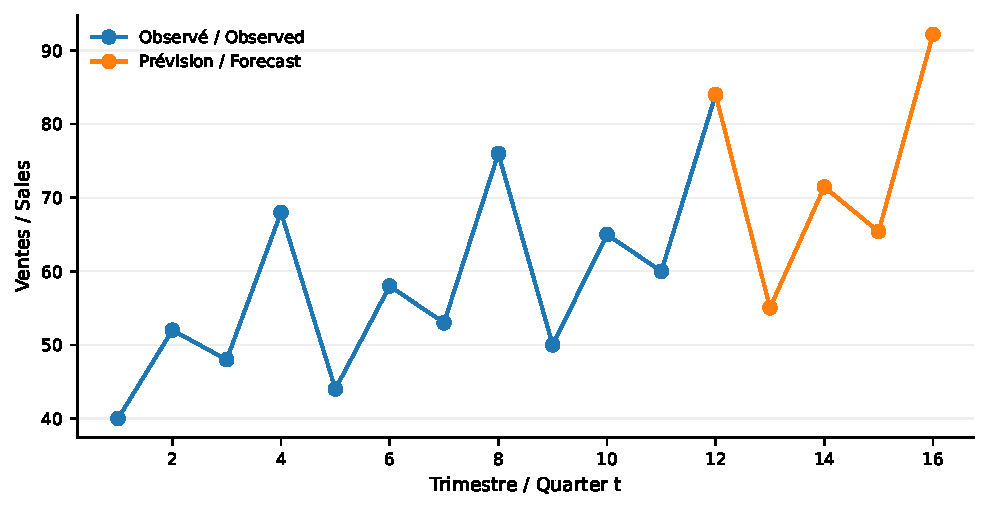
\includegraphics[width=0.82\textwidth,height=\textheight]{assets/chapter-5-solutions-en-datachart-01.pdf}

\emph{Ventes observées et prévisions 2022 / Observed and 2022 forecasts}

Check: the four normalised seasonal factors sum to 4. The 2022 forecasts are approximately 55.03, 71.46, 65.39 and 92.17.

\hypertarget{optional-advanced-practice}{%
\section{Optional advanced practice}\label{optional-advanced-practice}}

Explore additional interpretations and professional applications.

\emph{Advanced practice --- 15 min}

\hypertarget{exercise-4-forecast-evaluation}{%
\subsection{Exercise 4 -- Forecast evaluation}\label{exercise-4-forecast-evaluation}}

For this exercise, suppose actual 2008 values were {\(136,162,188,245\)}. Using the Exercise 3 forecasts, calculate forecast errors, MAE and RMSE, and explain the value of a separate validation period and a naive benchmark.

\hypertarget{fully-worked-solution-4}{%
\subsubsection{Fully worked solution}\label{fully-worked-solution-4}}

Forecasts are exactly those computed in exercise 3, without substituting rounded figures from another source.

\begin{longtable}[]{@{}llllll@{}}
\toprule\noalign{}
Q & Y & Prévision / Forecast & e=Y−Ŷ & \textbar e\textbar{} & e² \\
\midrule\noalign{}
\endhead
\bottomrule\noalign{}
\endlastfoot
1 & 136 & 133.655022 & 2.344978 & 2.344978 & 5.49892 \\
2 & 162 & 158.694123 & 3.305877 & 3.305877 & 10.92882 \\
3 & 188 & 191.552368 & -3.552368 & 3.552368 & 12.61932 \\
4 & 245 & 236.475885 & 8.524115 & 8.524115 & 72.66054 \\
\end{longtable}

\[MAE=(2.344978+3.305877+3.552368+8.524115)/4=4.431835.\]

\[RMSE=\sqrt{(2.344978^2+3.305877^2+(-3.552368)^2+8.524115^2)/4}=5.042509.\]

\[ME=(2.344978+3.305877-3.552368+8.524115)/4=2.655651.\]

The model underpredicts on average. Validation should be out of sample; a naive forecast is a useful benchmark.

\emph{Advanced practice --- 20 min}

\hypertarget{extra-1-forecast-validation-and-structural-break}{%
\subsection{Extra 1 --- Forecast validation and structural break}\label{extra-1-forecast-validation-and-structural-break}}

Actual monthly demand is 100, 104, 108, 150, 154 and 158. A trend model fitted on the first three months predicts 100, 104, 108, 112, 116 and 120.

\begin{enumerate}
\tightlist
\item
  Calculate forecast errors for months 4--6.
\item
  Calculate MAE and mean error over the validation period.
\item
  Diagnose the model.
\item
  Propose a responsible forecasting response.
\end{enumerate}

\textbf{Method hint:}

Use error = actual − forecast. A persistently positive error signals systematic underforecasting.

\hypertarget{fully-worked-solution-5}{%
\subsubsection{Fully worked solution}\label{fully-worked-solution-5}}

\textbf{Errors.} Month 4: 150−112 = 38; month 5: 154−116 = 38; month 6: 158−120 = 38.

\textbf{Validation metrics.} MAE = (38+38+38)/3 = \textbf{38}. Mean error is also \textbf{+38}, showing systematic underforecasting rather than random noise.

\textbf{Diagnosis.} The level jumps between months 3 and 4 while the subsequent slope remains close to four units per month. This is consistent with a level structural break. A model trained only before the break is obsolete.

\textbf{Response.} Investigate the business event causing the jump, re-estimate the level using post-break data, compare with a naive benchmark, retain a validation window, and issue prediction intervals. Do not simply average pre- and post-break observations without explaining the regime change.

\end{document}
